\documentclass{beamer}

\usepackage[T1]{fontenc}
\usepackage[utf8]{inputenc}
\usepackage[german]{babel}
\usepackage{multicol}

\usetheme{Warsaw}  %% Themenwahl
\usecolortheme{dolphin}
\title{Präsentation Simulation Drive Trough}

\author{L. Garstenauer S. Steininger S. Wernegger}
\date{\today}
 
\begin{document}
\maketitle
\frame{\tableofcontents[currentsection]}


\section{Aufgabenstellung}
\begin{frame} %%Eine Folie
  \frametitle{Aufgabenstellung} %%Folientitel
	\begin{itemize}
		\item Drive-Through-Schalter, bestehend aus Bestellbereich und Ausgabe
		\item Kunden Erstellung ist abhängig von der Tageszeit
		\item Falls Ausgabeschalter nicht frei ist muss gewartet werden
		\item Kunden können Umkehren wenn Wartezeit zu lang ist
		\item Falls das Essen nicht fertig ist muss darauf gewartet werden.
	\end{itemize}
\end{frame}

\section{Implementierung}
\begin{frame}
	 \frametitle{Implementierung } 
	 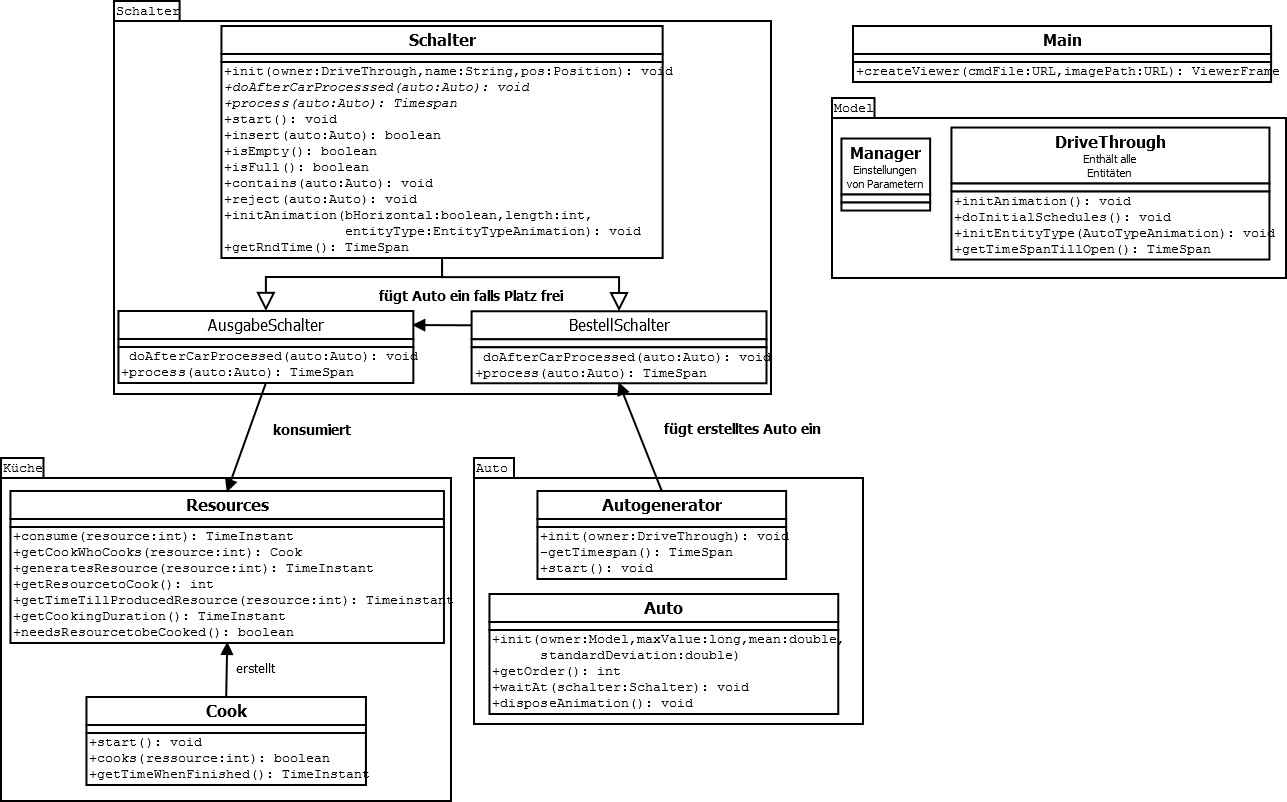
\includegraphics[width=\textwidth]{SimulationUML.png}
	 \begin{itemize}
	 \item []
	 \end{itemize}
	 
\end {frame}


\section{Was wurde getestet?}
\begin{frame} %%Eine Folie
  \frametitle{Was wurde getestet? } %%Folientitel
  Einfluss folgender Parameter auf die Kundenzufriedenheit und Wartezeit
  
 \begin{itemize}
 \item Länge der Warteschlangen Bestellung und Ausgabe
 \item Anzahl der Köche 
 \item Resourcenlimit
 \item Resourcenerstellungsdauer
 \item Anzahl verschiedener Ressourcen
 \item Dauer Bestellung und Ausgabe
 
 \end{itemize}
\end{frame}

\section{Was wurde Beobachtet?}
\begin{frame} %%Eine Folie
  \frametitle{Welche Resultate sind von Interesse } %%Folientitel

  
 \begin{itemize}
 \item Wartezeit im Drive Through gesamt
 \item Wartezeit am jeweiligen Schalter
 \item Durchschnittlicher Ressourcenvorrat
 \item Anzahl der unzufriedenen Kunden
 \item Zeit in der Köche untätig sind
 
 \end{itemize}
\end{frame}




\begin{frame} %%Eine Folie
  \frametitle{Kundenerstellungsverteilung } %%Folientitel
  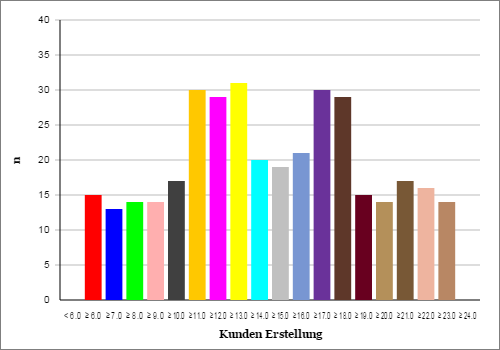
\includegraphics[width=\textwidth, height=0.85\textheight]{./Kunden.png}
 \begin{itemize}
 \item[]
 \item[]
 \end{itemize}
\end{frame}

\section{Ergebnisse}
\begin{frame} %%Eine Folie
  \frametitle{Ergebnisse} %%Folientitel
  \begin{itemize}
  	\item Auswirkungen des Ressourcenerstellung
  	\item Schalterbearbeitungsdauer
  	\item Auslastung der Köche
  \end{itemize}
\end{frame}


\begin{frame} %%Eine Folie
  \frametitle{ Auswirkungen des Ressourcenerstellung} 
  Auswirkung der Veränderung der jeweiligen Parameter
  die bei der Ressourcenerstellung beteiligt sind.\newline
  Veränderte Parameter:
  \begin{itemize}
  	\item Anzahl verschiedener Ressourcen
  	\item Ressourcenlimit
  	\item Ressourcenerstellungsdauer
  \end{itemize}
  
  Beobachtete Werte:
  \begin{itemize}
  	\item Ressourcenstand
  	\item Unzufriedene Kunden 
  	\item Wartezeit
  	\item Auslastung der Köche
  \end{itemize}
\end{frame}  

\begin{frame} %%Eine Folie
  \frametitle{Schalterbearbeitungsdauer} %%Folientitel
  Einfluss der Bearbeitungsdauer auf die Wartezeit\newline
  Veränderte Parameter:
  \begin{itemize}
  	\item Bestellung- /Ausgabedauer Verhältnis
  	\item Schalterlänge Ausgabe/Bestellung
  \end{itemize}
  Beobachtete Werte: %%bei folgender Folie auswertung es Reports 
  \begin{itemize}
  	\item Unzufriedene Kunden %Historgamm unzufrieden Kunden 
  	\item Wartezeit % Akkumulate Wartezeit %Queue bestellschater ausgabe zeile Kopieren warteschlange schalterbestellung und ausgabe
  	\item Wo haben Kunden das Drive-Through verlassen
  	%count Kunde verlässt ausgabe Bestellung
  \end{itemize}
\end{frame}

\begin{frame} %%Eine Folie
  \frametitle{Auslastung der Köche} %%Folientitel
	Veränderte Parameter:
  \begin{itemize}
  	\item Anzahl der Köche   	
  \end{itemize}
  
  Beobachtete Werte:
  \begin{itemize}
  	\item Ressourcenstand
  	\item Unzufriedene Kunden 
  	\item Wartezeit
  	\item Auslastung der Köche %queue unbeschäftige Köche
  \end{itemize}
\end{frame}

\section{Live - Demo}
\begin{frame} %%Eine Folie
  \frametitle{Live - Demo } %%Folientitel
  \begin{itemize}
  	\item Demonstration der Animation
  	\item Beispiel Report
  \end{itemize}
\end{frame}





\end{document}